\chapter{Image Classification}
In order for algorithms such as EMC to work, the amount of heterogeneity within the diffraction data set has to be limited [TOMAS is there an article describing this?]. Furthermore, each of the steps in the experiment introduces it own type of noise to the measured diffraction pattern. For example think of the debris clumping around small particles compared to the drop when sprayed with the GDVN, detector malfunctioning or saturation, or intensity fluctuations due to the random start of the SASE process. Often the results of the first two types of noise can not be tolerated by EMC, and image classification before the EMC step is necessary. Also fast feedback about the first type of noise is very useful to have during the experiment. So far a very robust sizing method has been developed, but more extended methods might come in useful. Several methods shown here can give rapid feedback on the heterogeneity of the particle.

\section{Template-based classification}
If your object has a known shape it could be possible to only select the diffraction patterns that are similar to a set of expected diffraction patterns from the object called templates. Paper III explores the possibility of template-based classification. In general this method is highly dependent on the choice of template, as well as the amount and type of variation present in your sample.

\section{Feature extraction}
Another way of selecting diffraction patterns is by extracting general features from the diffraction pattern such as size, particle shape, amount of saturation, number of particles in the beam. Based on the relative values associated with the features patterns might be selected or not, or the experimental conditions might be rapidly adjusted. This section describes several methods to extract features.

\subsection{Size}
A common method to determine the size of an object is fitting the central speckle to the central speckle of simulated diffraction pattern from a sphere. This method has shown to be successful for particles that have an icosahedral to spherical shape \cite{Hantke2014,Daurer2017}. If the 3rd to the 5th minima are also present in the diffraction pattern, the average of the 3rd-5th minima might be used to determine the size of the object as well. This method can be especially useful in case the central speckle or first minimum cannot be evaluated reliably due to for example saturation effects. Figure \ref{fig:sizing} shows the relative reliability of using different minima to assess the size of an icosahedral object. These results rely on simulated diffraction patterns \cite{Hantke2016}.

\begin{figure}[h]
\centering
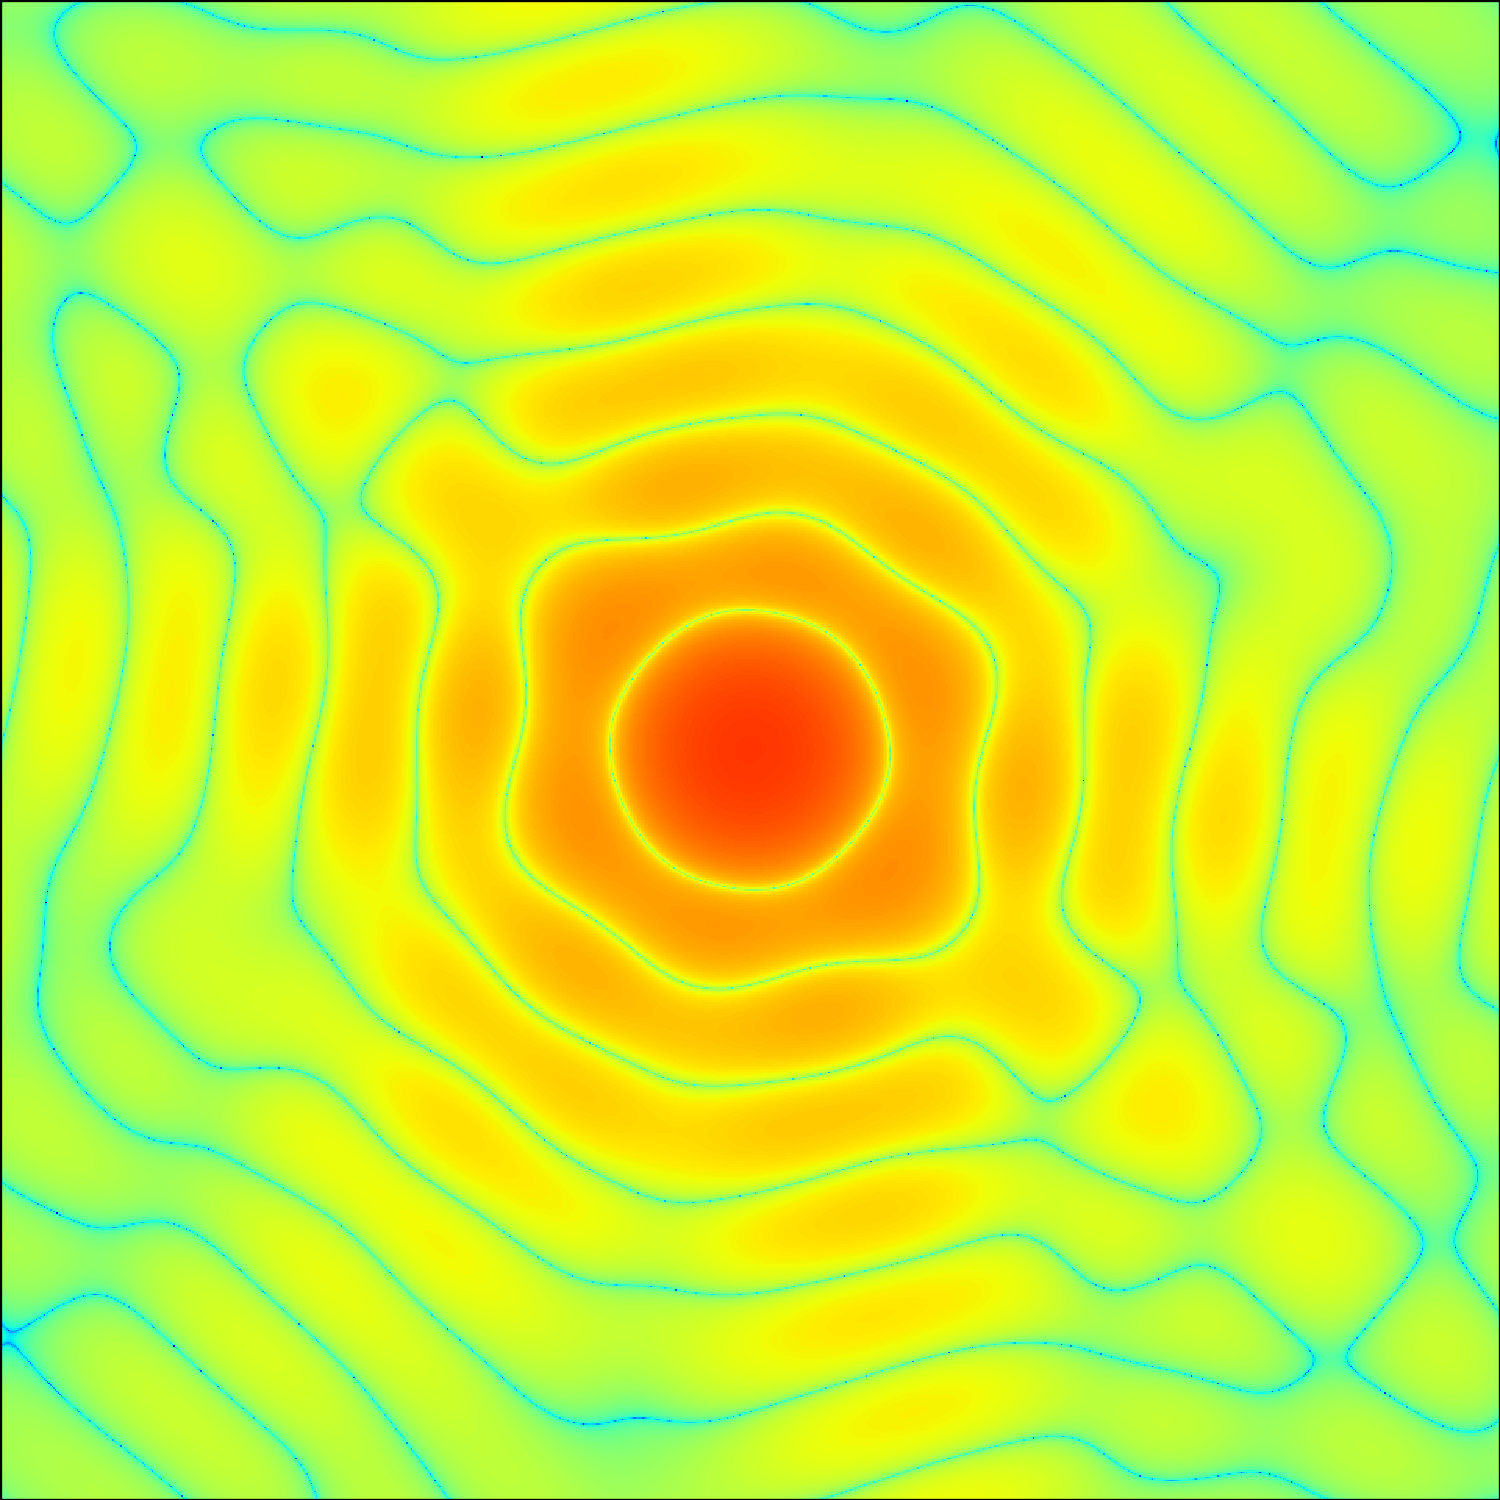
\includegraphics[width=42mm]{Chapter_08_ImageClassification_Simulated_Icosahedron.png}
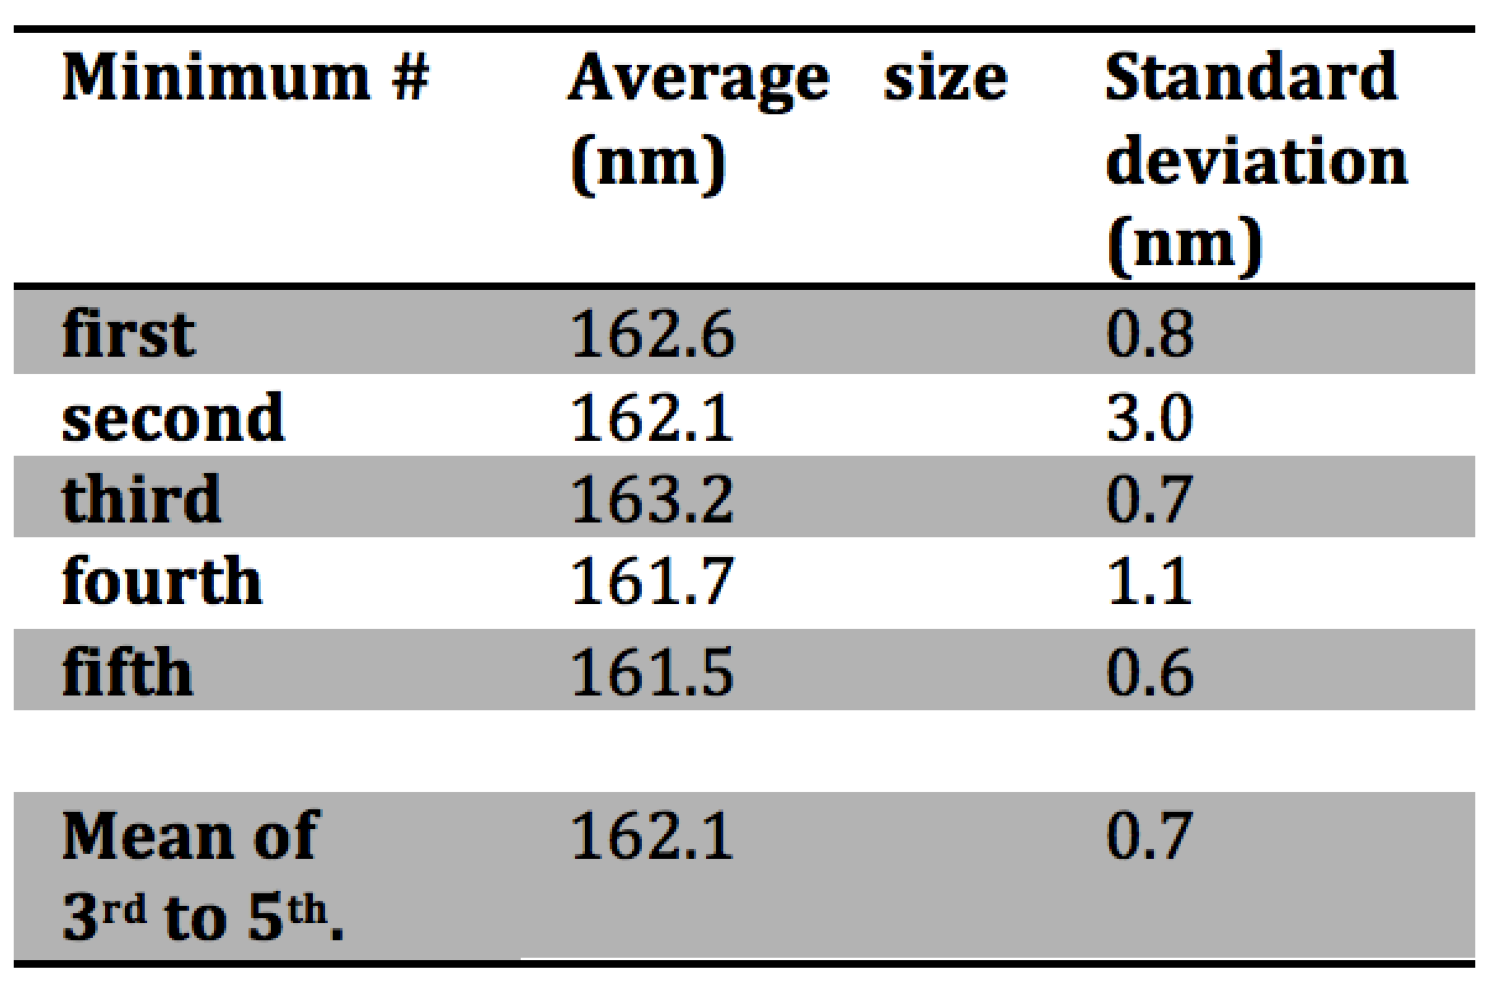
\includegraphics[width=65mm]{Chapter_08_ImageClassification_Stats.png}
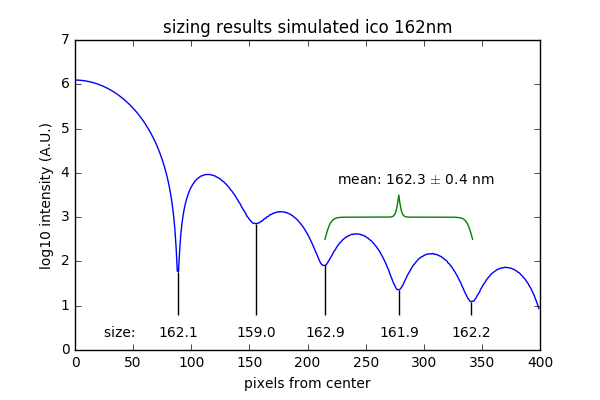
\includegraphics[width=100mm]{Chapter_08_ImageClassification_Sizing_Results.png}

\caption{}\label{fig:shape_assessment}
\end{figure}


\subsection{Edge detection}
Some objects are characterized by having sharp edges. A sharp edge in real space corresponds to a streak in the direction perpendicular to the edge in Fourier space. Objects and/or orientations of objects might be classified by determining if streaks are present, and how many. Figure explains the idea behind a streak finding algorithm described in paper IV.

\begin{figure}[h]
\centering
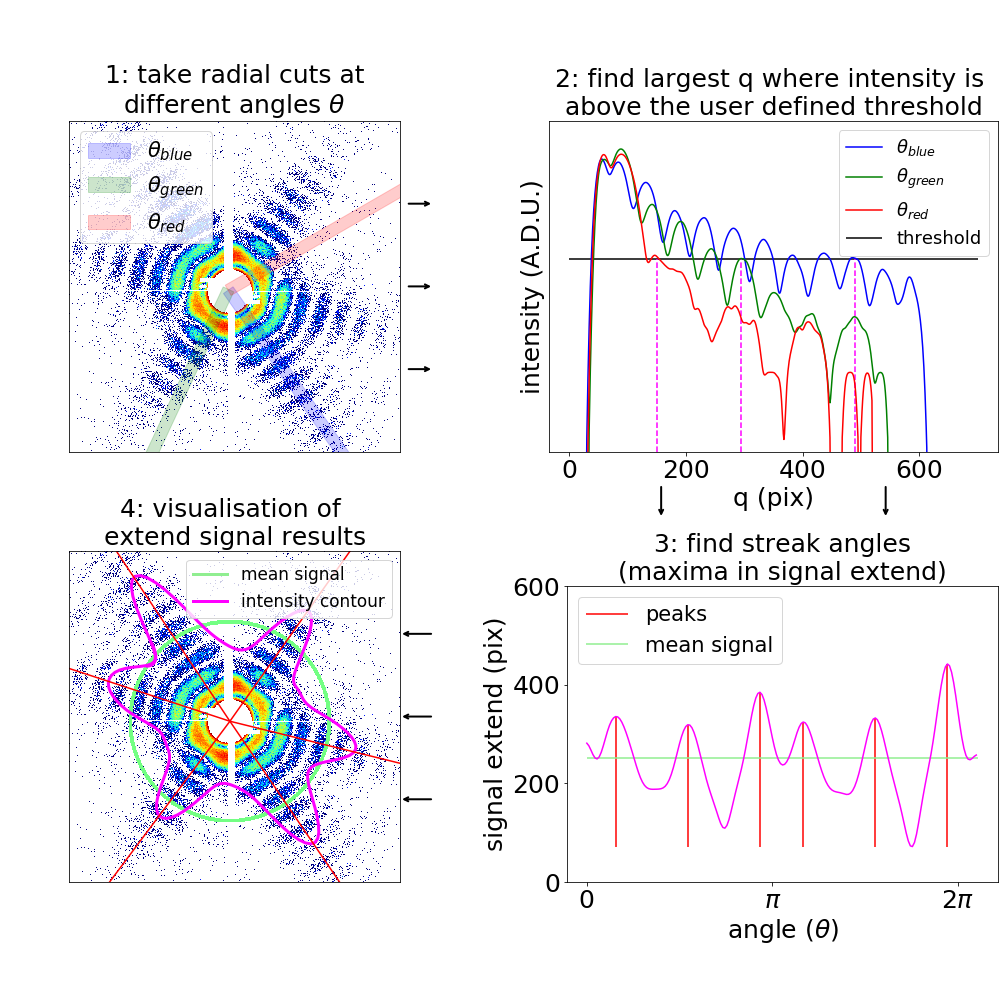
\includegraphics[width=120mm]{Chapter_08_ImageClassification_Edge_Detection.png}
\caption{}\label{fig:edge_detection}
\end{figure}

 
\subsection{Elongation}

It might also be possible to determine the elongation of the particle, either by evaluating the elongation of the central speckle \cite{Hantke2014,Daurer2017} or by evaluating the elongation of the central term in a filtered autocorrelation. This is useful in discerning between diffraction from spherical and non-spherical objects. The autocorrelation can only be used for convex objects. Figure 

\begin{figure}[h]
\centering
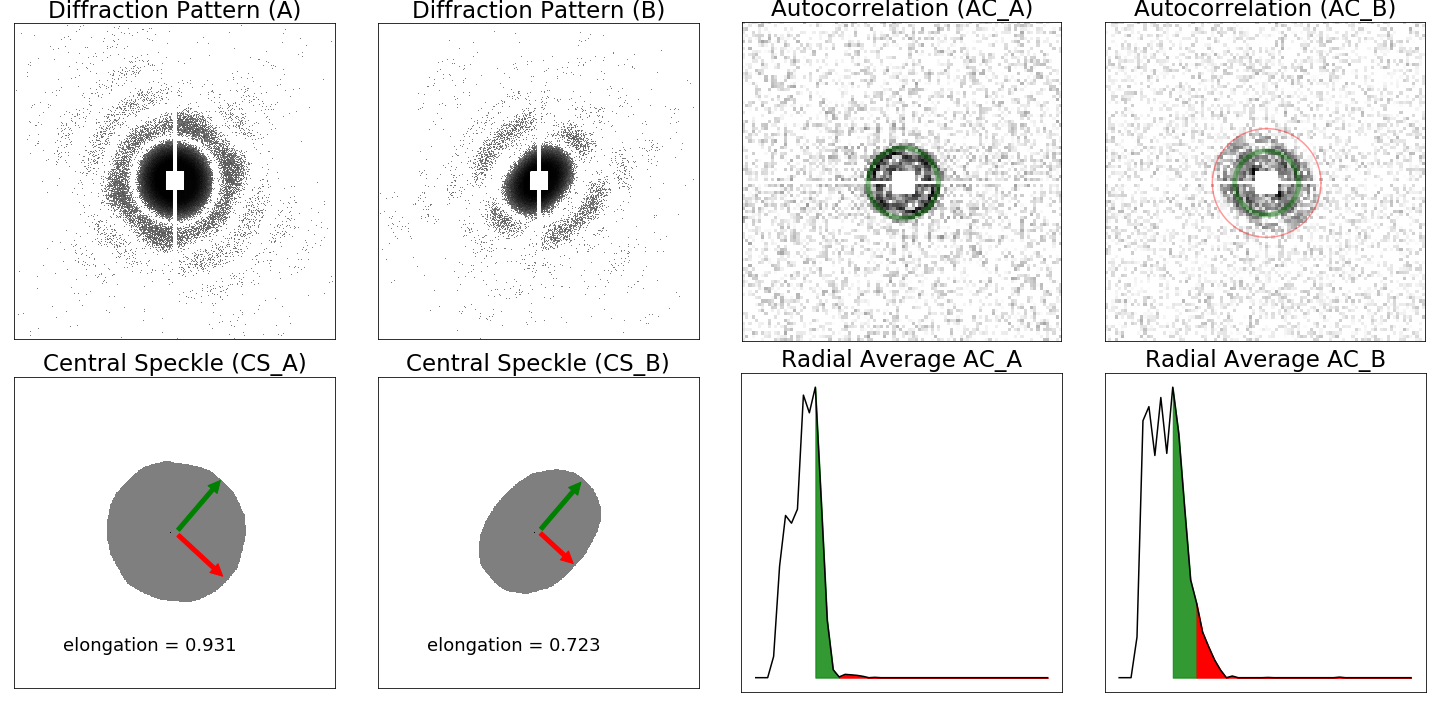
\includegraphics[width=120mm]{Chapter_08_ImageClassification_shape_assessment.png}
\caption{}\label{fig:shape_assessment}
\end{figure}


\subsection{The shape of the particle}
Particle shape or at least the particle size is important for automated phasing. So far automated routines have mainly dealt with icosahedral or round particles, as the size determined from the central speckle is enough to determine an accurate support constraint \cite{Hantke2014,Daurer2017}. The support size (and shape) of elongated particles such as most cells and many virus species cannot be accurately guessed in this way. This section introduces a method that can make a rough support guess for elongated particle by tracing the contour of the central term of the filtered autocorrelation. This method uses a Lorentz based edge detection, which basically defines the edge of an object as the steepest point in the gradient within the filtered autocorrelation.

\subsection{Multiple scatterers in the focus}

Due to the stochastic nature of the injection method, two particles can end up in the interaction region at the same time. If the particles are attached to each other, a similar pattern as seen in figure \ref{fig:shape_assessment} will occur. If the two pattern are separated in space, and so called Moire pattern will be observed (See Figure \ref{fig:moire_pattern}. These rings code for phase information, that simply can be retrieved from the autocorrelation, as shown in Paper XX. The resolution of the reconstruction will be related to the size scatterer, the amount of missing data, and the strength of the signal. Without going into detail as to why this is the case, it can be easily understood that such patterns should be separated from the patterns originating from single particles. This section describes a method that identifies patterns coming from multiple scatterers, be locating the non central terms in the autocorrelation (these are so-called holograms).
